%%%%%%%%%%%%%%%%%%%%%%%%%%%%%%%%%%%%%%%%%%%%%%%%%%%%%%%%%%%%%%%%%%%%%%%%%%%%%%%
% CAPÍTULO 1 – INTRODUÇÃO
%%%%%%%%%%%%%%%%%%%%%%%%%%%%%%%%%%%%%%%%%%%%%%%%%%%%%%%%%%%%%%%%%%%%%%%%%%%%%%%

\chapter{Introdução}
\label{sec:introducao}

Em nível estadual, o Tribunal de Justiça da Bahia (TJ-BA) mantém cerca de 24\,000 execuções penais ativas no Sistema Eletrônico de Execução Unificado (SEEU). Como a Lei de Execução Penal requer revisão trimestral e a Súmula 533 do Superior Tribunal de Justiça (STJ) confirma esse prazo, são necessários aproximadamente 8\,000 despachos por mês (\(\approx 267\) por dia) \cite{brasil1984lep,stj2015sumula533}.  
No Mutirão Processual Penal 2024 foram lançados 18\,600 atos em 60~dias, volume superior à meta fixada pela Portaria n.º 304/2024 do Conselho Nacional de Justiça (CNJ) e que evidencia sobrecarga \cite{tjba2024mutirao,cnj2024portaria304}.

Situação semelhante ocorreu no Tribunal de Justiça do Ceará (TJ-CE): a elaboração manual de 146 despachos consumiria mais de quatro horas, enquanto um robô executa cada um em 30~s \cite{tjce2023robos}. Esse panorama reforça a pertinência da \textit{pipeline} de \textit{Retrieval-Augmented Generation} (RAG) proposta, capaz de automatizar a busca semântica e gerar minutas, recuperando produtividade sem prejuízo à qualidade nem às garantias processuais.

A digitalização dos serviços públicos consolidou-se como pilar da modernização judicial, impulsionada por parcerias entre organismos internacionais e o Judiciário. O Programa das Nações Unidas para o Desenvolvimento (PNUD) e o CNJ, por exemplo, firmaram projetos que ampliam a transparência e o acesso à Justiça por meio de soluções digitais e governança inovadora \cite{undp2025pnudcnj}.

A experiência da Estônia evidencia o impacto de uma infraestrutura digital robusta na gestão de grandes volumes de informação pública: após a implantação do sistema e-Government, 98\,\% das declarações de imposto passaram a ser enviadas on-line em poucos minutos, e o mesmo percentual de empresas realiza seu registro por plataformas eletrônicas, aumentando a rastreabilidade e reduzindo fraudes \cite{divald2021eformalization}.  
Guardadas as devidas proporções, o SEEU enfrenta desafio semelhante — consolidar milhares de atos processuais dispersos e assegurar revisões trimestrais obrigatórias. O caso estoniano indica que a automação de consultas e a padronização digital podem gerar ganhos comparáveis de eficiência e transparência, reforçando a pertinência da \textit{pipeline} RAG aqui proposta.

Apesar desses avanços, a consulta manual a grandes acervos documentais permanece morosa e sujeita a erros, retardando decisões judiciais. Pesquisas sobre bancos de dados vetoriais demonstram que a indexação de documentos via \textit{embeddings} e a busca semântica reduzem significativamente a latência e aumentam a precisão na recuperação da informação \cite{taipalus2024vector,gao2023survey}.

As técnicas de RAG — que combinam inteligência artificial e grandes modelos de linguagem — despontam como solução para consultas em linguagem natural baseadas em documentos originais. Revisões recentes destacam seu potencial quando integradas a vetores de \textit{embeddings} para gerar respostas contextualizadas \cite{qwak2024integrating}, e estudos já aplicam variações de RAG a tarefas multimodais com resultados promissores \cite{pujiono2024implementing}.

Este trabalho propõe construir uma \textit{pipeline} RAG para o SEEU, implementada em Python, orquestrada por LangChain, exposta por meio de chatbot em Flask e empacotada em Docker para implantação consistente. Operadores do Direito poderão realizar buscas intuitivas e integrar a solução a sistemas externos por meio de API~REST.




%%%%%%%%%%%%%%%%%%%%%%%%%%%%%%%%%%%%%%%%%%%%%%%%%%%%%%%%%%%%%%%%%%%%%%%%%%%%%%%
% Seção 1.1 – Objetivos
%%%%%%%%%%%%%%%%%%%%%%%%%%%%%%%%%%%%%%%%%%%%%%%%%%%%%%%%%%%%%%%%%%%%%%%%%%%%%%%

\section{Objetivos}
\label{sec:objetivos}

\subsection{Objetivo Geral}
Desenvolver, para o Sistema Eletrônico de Execução Unificado (SEEU), uma \textit{pipeline} de \textit{Retrieval-Augmented Generation} (RAG) que automatize a recuperação e a disponibilização de dados públicos da execução penal, oferecendo interface conversacional (chatbot) e API~REST, a fim de modernizar os processos judiciais e ampliar a eficiência e a transparência da gestão.

\subsection{Objetivos Específicos}
\begin{enumerate}[label=\arabic*.]
  \item Coletar e organizar os dados públicos do SEEU, principalmente os documentos de suporte;
  \item Realizar a vetorização desses dados em um banco de dados vetorial (Elasticsearch, OpenSearch ou PostgreSQL+pgvector);
  \item Desenvolver uma pipeline que conecte o índice vetorial ao LLM selecionado, criando mecanismos para consultas precisas;
  \item Realizar testes de integração para avaliar a eficiência e a qualidade das respostas geradas;
  \item Criar uma interface de chatbot integrada à pipeline de RAG e ao LLM para interação em tempo real;
  \item Conduzir testes de usabilidade e implementar ajustes para aprimorar a experiência do usuário;
  \item Implementar uma API REST documentada para consumo externo;
  \item Preparar o ambiente para deployment, considerando aspectos de segurança e escalabilidade.
\end{enumerate}

%%%%%%%%%%%%%%%%%%%%%%%%%%%%%%%%%%%%%%%%%%%%%%%%%%%%%%%%%%%%%%%%%%%%%%%%%%%%%%%
% Seção 1.2 – Trabalhos Correlatos
%%%%%%%%%%%%%%%%%%%%%%%%%%%%%%%%%%%%%%%%%%%%%%%%%%%%%%%%%%%%%%%%%%%%%%%%%%%%%%%

\section{Trabalhos Correlatos}
\label{sec:trabalhos-correlatos}

Esta seção discute estudos que aplicam \textit{Retrieval-Augmented Generation} (RAG) a contextos jurídicos ou regulatórios, evidenciando avanços e limitações relevantes para o Sistema Eletrônico de Execução Unificado (SEEU).

\textbf{Edwards (2024)} apresenta um \textit{pipeline} RAG que integra grafos de conhecimento — construídos por especialistas e por LLMs — a uma base vetorial, automatizando relatórios de acreditação AACSB. O roteamento de consultas, a decomposição em subconsultas e a síntese automática de respostas reduzem o esforço humano e aumentam a transparência; entretanto, a curadoria desses grafos ainda exige validação manual \cite{edwards2024hybrid}.  
\emph{Relação com o SEEU}: o sistema proposto neste TCC adota roteamento e síntese similares, mas aplica regras jurídicas automáticas para validar o grafo, minimizando a intervenção humana.

\textbf{Pujiono, Agtyaputra e Ruldeviyani (2024)} implementam um chatbot que combina \textit{embeddings} da OpenAI, armazenamento vetorial no Pinecone e geração condicionada à recuperação, respondendo a perguntas sobre normas de agências públicas. O estudo comprova a utilidade do RAG na interpretação de regulamentos, porém não trata acervos processuais volumosos \cite{pujiono2024implementing}.  
\emph{Relação com o SEEU}: o presente trabalho incorpora técnicas de indexação escalável e métricas de cobertura para manipular milhares de peças processuais e atender às revisões trimestrais obrigatórias.

\textbf{Aquino (2024)} descreve um fluxo RAG local para extrair informações estruturadas de documentos de licitação, utilizando \textit{embeddings} BERTimbau, Chroma como \textit{vector store} e LLMs \textit{open source}. O autor relata ganhos de precisão sobre técnicas tradicionais, mas alerta para o elevado custo computacional \cite{aquino2024extracting}.  
\emph{Relação com o SEEU}: esta pesquisa adota estratégias de compressão e particionamento que reduzem o consumo de recursos, viabilizando a execução em infraestrutura de tribunal estadual sem comprometer a qualidade das respostas.

%%%%%%%%%%%%%%%%%%%%%%%%%%%%%%%%%%%%%%%%%%%%%%%%%%%%%%%%%%%%%%%%%%%%%%%%%%%%%%%
% Seção 1.3 – Solução Proposta
%%%%%%%%%%%%%%%%%%%%%%%%%%%%%%%%%%%%%%%%%%%%%%%%%%%%%%%%%%%%%%%%%%%%%%%%%%%%%%%

\section{Solução Proposta}
\label{sub:solucao-proposta}

A solução consiste em uma \textit{pipeline} RAG organizada nos seguintes módulos:

\begin{itemize}[label=\textbullet]
  \item \textbf{Coleta automática} de documentos oficiais (PDF) do SEEU;
  \item \textbf{Pré-processamento} — limpeza, OCR e segmentação em \emph{chunks};
  \item \textbf{Vetorização} e indexação em base vetorial (FAISS ou OpenSearch);
  \item \textbf{Orquestração} via LangChain, com fallback híbrido (keyword + semantic);
  \item \textbf{Interface conversacional} (chatbot) e \textbf{API REST} documentada em OpenAPI;
  \item \textbf{Camada de validação jurídica} para reduzir alucinações;
  \item \textbf{Testes automatizados} de integração e regressão (precisão, recall, F1);
  \item \textbf{Monitoramento e métricas} (tempo de resposta, taxa de erro, taxa de alucinação);
  \item \textbf{Segurança e controle de acesso} (JWT, HTTPS, LGPD);
  \item \textbf{Deployment conteinerizado} (Docker/Kubernetes) com CI/CD;
  \item \textbf{Documentação técnica completa} (código-fonte comentado, manuais, API);
  \item \textbf{Plano de mitigação de riscos} e atualização contínua de dependências.
\end{itemize}



%%%%%%%%%%%%%%%%%%%%%%%%%%%%%%%%%%%%%%%%%%%%%%%%%%%%%%%%%%%%%%%%%%%%%%%%%%%%%%%
% CAPÍTULO 2 – FUNDAMENTAÇÃO TEÓRICA E REVISÃO DE LITERATURA
%%%%%%%%%%%%%%%%%%%%%%%%%%%%%%%%%%%%%%%%%%%%%%%%%%%%%%%%%%%%%%%%%%%%%%%%%%%%%%%

% ============================================================
\chapter{Fundamentação Teórica e Revisão de Literatura}
\label{chap:fundamentacao_literatura}

\section{Bancos de Dados Vetoriais}
\label{sec:bancos-vetoriais}

\subsection{Definição}
Bancos de dados vetoriais são sistemas especializados em armazenar, indexar e
consultar vetores em espaço multidimensional. Esses vetores — denominados
\emph{embeddings} — são gerados por modelos de \emph{machine learning} e
capturam características semânticas de dados não estruturados, como texto,
imagens, áudio e vídeo \cite{qwak2024integrating}.

\subsection{Importância}
A busca por similaridade em embeddings é fundamental para diversas
aplicações:
\begin{itemize}
  \item \textbf{Sistemas de recomendação} – identificação de itens similares às preferências do usuário;
  \item \textbf{Busca semântica} – consultas que interpretam o significado das palavras, não apenas correspondências exatas;
  \item \textbf{Reconhecimento de padrões} – detecção de faces, objetos ou outros padrões em grandes volumes de dados;
  \item \textbf{Pipelines de IA} – armazenamento eficiente de embeddings utilizados por modelos de \emph{deep learning}.
\end{itemize}
Tais bases oferecem consultas rápidas, baixa latência e alta escalabilidade —
qualidades essenciais em \emph{NLP}, visão computacional e outros domínios que
envolvem grandes conjuntos de dados não estruturados
\cite{qwak2024integrating}.

\subsection{Análise comparativa de soluções}
\begin{description}
  \item[Elasticsearch:] plataforma distribuída e escalável com suporte a busca vetorial pelo \texttt{Elastic Vector Search}. Limitação: implementação vetorial ainda pouco madura em alta dimensionalidade.

  \item[OpenSearch:] \emph{fork} aberto do Elasticsearch com recursos vetoriais nativos e manutenção comunitária. Limitação: requer ajustes finos para consultas complexas.

  \item[PostgreSQL + \texttt{pgvector}:] integra dados relacionais e vetoriais em um mesmo SGBD. Limitação: desempenho inferior em buscas de larga escala.

  \item[Milvus:] banco vetorial especializado, otimizado para similaridade e escalável a bilhões de vetores. Limitação: maior complexidade de configuração e manutenção.

  \item[FAISS:] biblioteca de alto desempenho amplamente utilizada em pesquisa. Limitação: não é um SGBD completo, exigindo integração adicional.

  \item[Weaviate:] código aberto que combina buscas vetoriais e de grafo, permitindo consultas semânticas e relacionais. Limitação: requer \emph{tuning} avançado para desempenho ótimo.

  \item[Oracle Vector DB:] integração nativa ao ecossistema Oracle, com alta performance e segurança empresarial. Limitação: licenciamento oneroso e menor flexibilidade frente a soluções abertas \cite{oracle2025vector}.

  \item[IBM Vector DB:] forte integração com ferramentas de IA da IBM, oferecendo recursos robustos de análise vetorial. Limitação: custo elevado e configuração complexa \cite{ibm2025vector}.
\end{description}

%--------------------------------------------------------------------
% ------------------------------------------------------------
\section{Large Language Models (LLMs)}
\label{sec:llm}

\subsection*{INTRODUÇÃO}
Os Modelos de Linguagem de Grande Porte (LLMs), baseados na arquitetura
Transformer \cite{vaswani2017attention,naveeda2024comprehensive}, elevaram o
estado da arte em Processamento de Linguagem Natural (PLN), permitindo síntese,
tradução e interpretação semântica de documentos em larga escala. No Sistema
Eletrônico de Execução Unificado (SEEU), essas redes neurais substituem buscas
puramente lexicais por consultas semânticas, aumentando a agilidade e a
precisão das respostas. A integração de LLMs a bancos de dados vetoriais
\cite{taipalus2024vector,qwak2024integrating} reforça essa capacidade,
fornecendo resultados contextualizados a partir de extensos acervos
documentais.

\subsection*{ASPECTOS TÉCNICOS}
\begin{enumerate}[label=\textbf{2.\arabic*}, leftmargin=*]
  \item \textbf{PRE-TRAINING}\label{itm:pretraining}\\
        O modelo é submetido a um corpus genérico e volumoso para capturar
        padrões linguísticos amplos, formando uma base de conhecimento
        diversificada \cite{naveeda2024comprehensive}.
  
  \item \textbf{FINE-TUNING}\label{itm:finetuning}\\
        Realiza-se \emph{fine-tuning} com dados jurídicos da execução penal.
        Estratégias de regularização (e.g., \textit{dropout}, \textit{early
        stopping}) evitam \textit{overfitting}. A eficácia é medida por
        precisão, \textit{recall} e F1-score
        \cite{yue2023disclawllm,lai2023lawm}.
  
  \item \textbf{DESAFIOS TÉCNICOS}\label{itm:desafios}\\[-0.8em]
        \begin{itemize}
          \item Limpeza de dados — normalização de peças processuais;
          \item Seleção de hiperparâmetros — equilíbrio entre desempenho e custo;
          \item Escalabilidade — baixa latência com grandes volumes documentais
                \cite{edwards2024hybrid,pujiono2024implementing,aquino2024extracting}.
        \end{itemize}
  
  \item \textbf{VALIDAÇÃO E RESULTADOS ESPERADOS}\label{itm:validacao}\\
        A avaliação inclui: (i) precisão na recuperação de informações;
        (ii) qualidade das respostas validadas por especialistas; e
        (iii) eficiência computacional face aos métodos atuais do SEEU.
        Resultados preliminares indicam ganhos expressivos de precisão e
        \textit{recall}.
\end{enumerate}

\subsection*{CONSIDERAÇÕES FINAIS}
A combinação de \ref{itm:pretraining}–\ref{itm:validacao}, aliada a bancos
vetoriais, constitui abordagem inovadora para consultas jurídicas, reduzindo
prazos e aumentando a transparência do Judiciário
\cite{belarmino2025aplicacao,divald2021eformalization}. Estudos futuros podem
estender a metodologia a outros ramos do Direito, consolidando a transformação
digital no setor público.

%--------------------------------------------------------------------
\section{Retrieval-Augmented Generation (RAG)}
\label{sec:rag}

\subsection{Introdução}
\textit{Retrieval-Augmented Generation} (RAG) associa a competência de
\textit{Large Language Models} (LLMs) em gerar texto à recuperação automática de
documentos, reduzindo \textit{alucinações} ao fundamentar as respostas em
evidências externas verificáveis
\cite{lewis2020rag,gao2023survey,edwards2024hybrid,pujiono2024implementing}.
LLMs armazenam conhecimento nos parâmetros (\emph{memória paramétrica}); já o
RAG adiciona uma \emph{memória não paramétrica} consultável em tempo real,
essencial em cenários como o SEEU, cujo acervo documental é volumoso e
dinâmico.

\subsection{Fundamentos}
\textbf{Data retrieval.} Consultas e documentos são convertidos em
\emph{embeddings}; métodos densos, como o \textit{Dense Passage Retrieval}
(DPR), aproximam vetores por similaridade de cosseno ou distância euclidiana,
retornando um subconjunto $k$-relevante
\cite{lewis2020rag,taipalus2024vector,mageirakos2025cracking}.\\
\textbf{Content generation.} Um modelo \emph{encoder--decoder} (ex.: BART ou
T5) concatena os trechos recuperados ao \textit{prompt} e gera a resposta. O
treinamento conjunto (Sec.~\ref{sec:rag:pipeline}) ensina o \textit{retriever}
a apresentar evidências úteis ao gerador
\cite{aquino2024extracting,belarmino2025aplicacao}.

\subsection{Pipeline}
\label{sec:rag:pipeline}
\begin{enumerate}[label=\arabic*.]
  \item \textbf{Ingestion} – extração de fontes estruturadas (bases SQL, CKAN)
        e não estruturadas (PDF, HTML); limpeza, segmentação em parágrafos e
        criação de embeddings com modelos como \textit{all-MiniLM}.
        Objetos $\langle\text{ID},\,\text{embedding},\,\text{metadata}\rangle$
        são indexados em repositórios vetoriais (FAISS, Pinecone)
        \cite{qwak2024integrating,taipalus2024vector}.
  \item \textbf{Retrieval} – a consulta é vetorizada e comparada com o índice;
        top-$k$ documentos são ranqueados. Estratégias \emph{re-rank} com
        \textit{cross-encoders} ou fusão heurística (ex.: \textit{Reciprocal
        Rank Fusion}) aumentam precisão \cite{edwards2024hybrid}.
  \item \textbf{Treinamento conjunto} – ajuste \textit{end-to-end} de
        \textit{retriever} e \textit{generator} via
        \textit{maximum-likelihood} ou \textit{policy-gradient}, fazendo o
        \textit{retriever} maximizar a probabilidade da resposta correta
        \cite{zhang2025fine}.
\end{enumerate}

\subsection{Variantes}
\begin{itemize}
  \item \textbf{RAG-Sequence} – cada hipótese de documento gera uma resposta
        completa; a probabilidade final marginaliza sobre o conjunto recuperado
        \cite{lewis2020rag,edwards2024hybrid}.
  \item \textbf{RAG-Token} – a distribuição é recalculada a cada token,
        permitindo que diferentes documentos contribuam ponto a ponto; amplia a
        cobertura factual, mas exige mecanismos de coerência global
        \cite{zhang2025fine}.
\end{itemize}

\subsection{Desafios e limitações}
\begin{itemize}
  \item \textbf{Latência} – cada consulta envolve busca vetorial $+$ geração,
        podendo ultrapassar limites de tempo real
        \cite{scalable2025overload}.
  \item \textbf{Atualização em tempo real} – garantir que o índice reflita
        alterações frequentes do corpus demanda pipelines de reingestão
        contínua \cite{taipalus2024vector}.
  \item \textbf{Qualidade da recuperação} – ruído ou pouca cobertura no índice
        reduz acurácia; técnicas de \textit{negative-sampling} e \textit{hard
        negatives} no treinamento mitigam o problema
        \cite{gao2023survey,salemi2024hallucination}.
  \item \textbf{Coerência textual} – fusão de múltiplas fontes pode gerar
        redundância ou mudança de estilo; pós-edição automática e
        penalidades de repetição auxiliam \cite{zhang2025fine}.
\end{itemize}

% ------------------------------------------------------------
\section{Programa das Nações Unidas para o Desenvolvimento (PNUD)}
\label{sec:pnud}

O Programa das Nações Unidas para o Desenvolvimento (PNUD) é a agência da
Organização das Nações Unidas (ONU) responsável por promover o desenvolvimento
humano sustentável e erradicar a pobreza em mais de 170 países e territórios
\cite{undp2025sobre,undp2025onu}. Sediado em Nova York, o PNUD oferece suporte
técnico e financeiro a políticas públicas voltadas às populações mais
vulneráveis.

\subsection{Objetivos e mandato}
O mandato do PNUD abrange quatro eixos centrais:
\begin{itemize}
  \item \textbf{Erradicação da pobreza} – programas para reduzir a pobreza
  extrema e melhorar as condições de vida;
  \item \textbf{Desigualdade e inclusão social} – políticas que promovem
  igualdade de oportunidades;
  \item \textbf{Desenvolvimento sustentável} – iniciativas que conciliam o uso
  de recursos naturais e a proteção ambiental;
  \item \textbf{Governança democrática} – fortalecimento institucional,
  transparência e participação cidadã.
\end{itemize}
Tais ações alinham-se à Agenda~2030 e aos Objetivos de Desenvolvimento
Sustentável (ODS), sobretudo o ODS~1 (pobreza) e o ODS~10 (redução das
desigualdades) \cite{wikipedia2025pnud}.

\subsection{Estrutura e funcionamento}
Financiado por contribuições voluntárias de Estados-membros, setor privado e
ONGs, o PNUD é chefiado por um Administrador indicado pelo Secretário-Geral da
ONU e aprovado pela Assembleia Geral \cite{undp2025onu}. No Brasil, opera em
parceria com governos, sociedade civil e empresas, direcionando projetos que
fomentam o desenvolvimento sustentável e reduzem desigualdades
\cite{undp2025sobre}.

% ------------------------------------------------------------
\section{Parceria CNJ–PNUD: direitos humanos e acesso à justiça}
\label{sec:cnj-pnud}

Em 2025, o Conselho Nacional de Justiça (CNJ) e o PNUD firmaram acordo de
cooperação para fortalecer o Poder Judiciário na promoção de direitos humanos,
sustentabilidade socioambiental e acesso à justiça por populações
vulnerabilizadas \cite{undp2025pnudcnj}. O projeto complementa iniciativas como:
\begin{itemize}
  \item \textbf{Programa Justiça 4.0} – transformação digital do Judiciário
        brasileiro, ampliando transparência e celeridade processual;
  \item \textbf{Fazendo Justiça} – melhorias nas políticas de privação de
        liberdade e reintegração social.
\end{itemize}

A juíza auxiliar Karen Luise destaca que a ação se alinha à Estratégia 2021-2026
do CNJ, priorizando igualdade e acesso jurisdicional. Para o PNUD, a parceria
reforça o ODS~16, que visa instituições eficazes e inclusivas
\cite{undp2025pnudcnj}. As atividades previstas contemplam:
\begin{enumerate}
  \item fortalecimento institucional e capacitação de magistrados;
  \item diagnósticos situacionais e desenvolvimento de metodologias inclusivas;
  \item projetos-piloto focados em crianças e adolescentes em abrigamento,
        mulheres, pessoas LGBTQIA$+$, povos indígenas, pessoas em situação de
        rua, idosos, pessoas com deficiência e grupos vulneráveis por fatores
        socioambientais ou raciais.
\end{enumerate}

\subsection*{Impacto esperado}
O fortalecimento do sistema judiciário — por meio da digitalização,
capacitação e práticas inovadoras — tende a ampliar o acesso efetivo à justiça e
a reduzir barreiras estruturais. A cooperação CNJ–PNUD, portanto, contribui para
o cumprimento dos compromissos internacionais do Brasil relacionados aos ODS,
promovendo uma sociedade mais justa e inclusiva
\cite{undp2025pnudcnj}.



%%%%%%%%%%%%%%%%%%%%%%%%%%%%%%%%%%%%%%%%%%%%%%%%%%%%%%%%%%%%%%%%%%%%%%%%%%%%%%%
% CAPÍTULO 3 – TECNOLOGIAS (revisado)
%%%%%%%%%%%%%%%%%%%%%%%%%%%%%%%%%%%%%%%%%%%%%%%%%%%%%%%%%%%%%%%%%%%%%%%%%%%%%%%

\chapter{Tecnologias}
\label{chap:tecnologias}

\section{Linguagem e Bibliotecas Principais}
\begin{itemize}[label=\textbullet]
  \item \textbf{Python} – linguagem base, com extensas bibliotecas para NLP e ML (\cite{python2024});
  \item \textbf{Pandas} – manipulação de dados tabulares e pré-processamento de textos (\cite{pandas2024});
  \item \textbf{NumPy} – operações vetoriais e matrizes de alto desempenho.
\end{itemize}

\section{Indexação e Recuperação Vetorial}
\subsection{OpenSearch}
Mecanismo de busca distribuída com suporte nativo a buscas vetoriais via plugins; ótimo para cenários de alta disponibilidade e grandes volumes de dados (\cite{taipalus2024vector}).

\subsection{FAISS}
Biblioteca de similaridade aproximada desenvolvida pelo Facebook, altamente otimizada para bilhões de vetores, mas depende de um sistema auxiliar para metadados e persistência (\cite{facebookresearch2024faiss}).

\subsection{Milvus e Weaviate}
Soluções especializadas de código-aberto com integração a grafos (Weaviate) e suporte a esquemas de indexação avançados (Milvus). Indicadas para aplicações críticas de IA.

\section{Modelos de Linguagem}
\subsection{LLama}
Modelo open-source eficiente, customizável para domínios específicos, incluindo jurídico.

\subsection{Hugging Face Transformers}
Framework que fornece acesso a dezenas de modelos pré-treinados, tokenizadores e utilitários de pipeline (\cite{huggingface2024}).

\section{Orquestração de Pipeline}
\subsection{LangChain}
Framework modular que conecta retriever (FAISS/OpenSearch) e generator (LLM), permitindo composição de fluxos e gerenciamento de prompts (\cite{langchain2024}).

\subsection{Controle de Prompt e Fallback}
Implementação de lógica para reformulação de prompts e fallback a dados oficiais caso o LLM retorne resposta vaga.

\section{Infraestrutura e Deployment}
\subsection{Docker e Kubernetes}
Containerização para padronização de ambientes e orquestração em cluster, garantindo escalabilidade horizontal e isolamento.

\subsection{API REST com Flask}
Microframework escolhido pela maturidade e simplicidade, expondo endpoints para chatbot e integração externa (\cite{flask2024}).


%%%%%%%%%%%%%%%%%%%%%%%%%%%%%%%%%%%%%%%%%%%%%%%%%%%%%%%%%%%%%%%%%%%%%%%%%%%%%%%
% CAPÍTULO 4 – METODOLOGIA (revisado)
%%%%%%%%%%%%%%%%%%%%%%%%%%%%%%%%%%%%%%%%%%%%%%%%%%%%%%%%%%%%%%%%%%%%%%%%%%%%%%%

\chapter{Metodologia}
\label{chap:metodologia}

\section{Arquitetura da Pipeline}
A pipeline combina quatro estágios principais: ingestão, pré‐processamento, indexação e geração. Cada estágio é containerizado e orquestrado via Kubernetes (Figura~\ref{fig:arquitetura_pipeline}).

\section{Coleta de Dados}
\begin{itemize}[label=\textbullet]
  \item Raspagem automática dos portais do CNJ usando Python e bibliotecas como \texttt{requests} e \texttt{BeautifulSoup};
  \item Agendamento via \emph{cron} ou Airflow para verificações diárias de novos documentos.
\end{itemize}

\section{Pré-processamento e Segmentação}
\begin{enumerate}[label=\arabic*.]
  \item Conversão de PDF para texto com \texttt{pdfplumber};
  \item Remoção de cabeçalhos, rodapés e caracteres especiais;
  \item Divisão em \emph{chunks} de 500--1000 tokens para otimizar a busca local.
\end{enumerate}

\section{Engenharia de Embeddings}
Escolha de modelo de embedding (BERTimbau ou OpenAI), parametrização de tamanho e normalização para garantir coerência semântica.

\section{Indexação e Armazenamento}
\begin{itemize}[label=\textbullet]
  \item Indexação dos embeddings em OpenSearch/FAISS com metadados (origem, data, posição);
  \item Definição de métricas de similaridade (cosine similarity) e thresholds de corte.
\end{itemize}

\section{Orquestração e Consulta}
Implementação em LangChain:
\begin{itemize}[label=\textbullet]
  \item Conversão da consulta em embedding;
  \item Recuperação dos top-k \emph{chunks};
  \item Geração da resposta pelo LLM, mesclando múltiplas fontes se necessário (\emph{RAG-Token}).
\end{itemize}

\section{Desenvolvimento do Chatbot e da API}
\begin{itemize}[label=\textbullet]
  \item Chatbot baseado em WebSocket para interação síncrona;
  \item Endpoints RESTful em Flask para consultas e feedback de usabilidade.
\end{itemize}

\section{Avaliação e Métricas}
\begin{itemize}[label=\textbullet]
  \item Precisão, recall e F1-Score em um conjunto de questões de benchmark (fase de testes);
  \item Ensaios de usabilidade qualitativos com operadores do Direito para avaliar intuitividade e confiança.
\end{itemize}

\section{MLOps e Monitoramento}
\begin{itemize}[label=\textbullet]
  \item Pipelines de CI/CD para build e deploy automáticos;
  \item Monitoramento de latência e acurácia em produção, com alertas para queda de desempenho;
  \item Feedback loop para re-treinamento periódico com dados reais de uso.
\end{itemize}

\begin{figure}[h!]
  \centering
  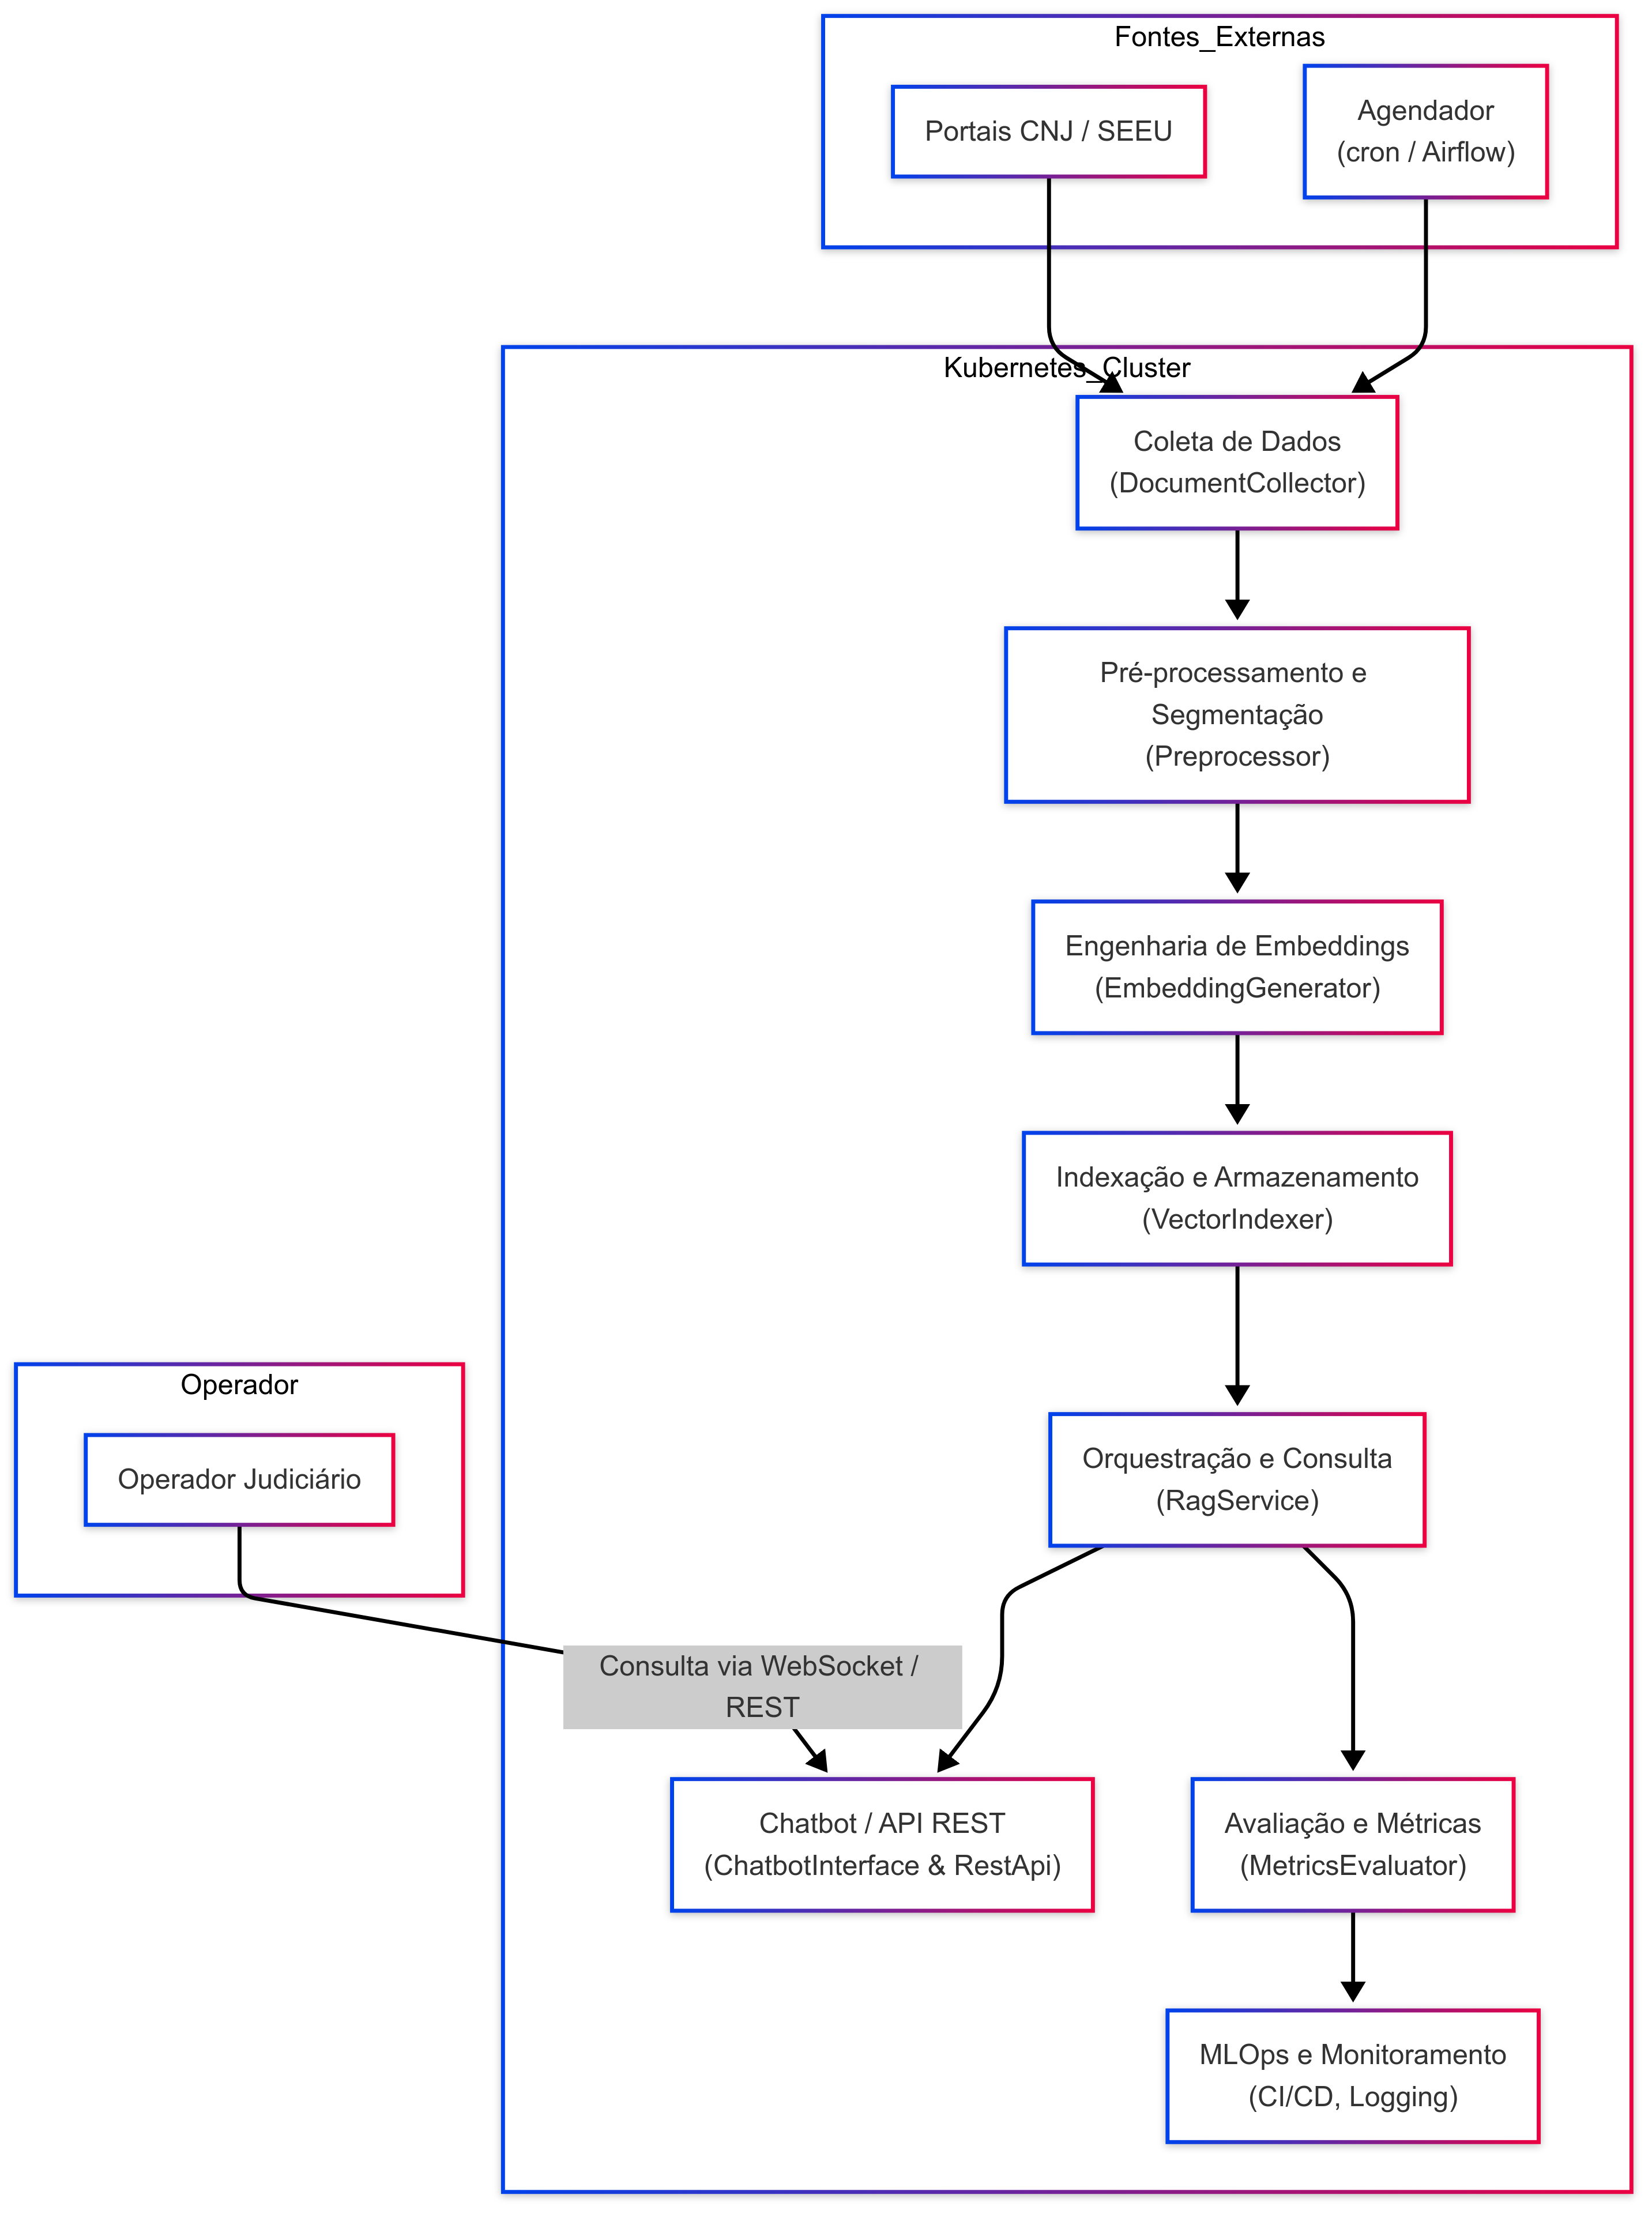
\includegraphics[width=0.8\textwidth]{04-figuras/arquitetura_pipeline.png}
  \caption{Arquitetura geral da pipeline RAG.}
  \label{fig:arquitetura_pipeline}
\end{figure}


%%%%%%%%%%%%%%%%%%%%%%%%%%%%%%%%%%%%%%%%%%%%%%%%%%%%%%%%%%%%%%%%%%%%%%%%%%%%%%%
% CAPÍTULO 5 – RESULTADOS ESPERADOS
%%%%%%%%%%%%%%%%%%%%%%%%%%%%%%%%%%%%%%%%%%%%%%%%%%%%%%%%%%%%%%%%%%%%%%%%%%%%%%%

\chapter{Resultados Esperados}
\label{chap:resultados}

Este capítulo descreve, de forma detalhada, os resultados que se almeja alcançar com a execução do presente Trabalho de Conclusão de Curso (TCC). Tais resultados derivam dos objetivos estabelecidos no Capítulo~\ref{sec:objetivos} e da metodologia apresentada no Capítulo~\ref{chap:metodologia}, respeitando as normas da Associação Brasileira de Normas Técnicas -- ABNT (NBR 14724:2011) para trabalhos acadêmicos.

\section{Implementação de uma pipeline RAG funcional}
Espera-se disponibilizar uma pipeline de \emph{Retrieval-Augmented Generation} (RAG) plenamente operacional, capaz de integrar um modelo de linguagem de grande porte (LLM) a um índice vetorial que contenha os documentos públicos do Sistema Eletrônico de Execução Unificado (SEEU). A solução deverá oferecer uma interface conversacional (chatbot) em língua portuguesa, além de uma API REST para consumo externo, permitindo consultas em linguagem natural e retornando respostas fundamentadas nos documentos originais.

\section{Ganho de eficiência na recuperação de informações}
A implementação proposta deverá reduzir o tempo médio despendido pelos operadores do Direito para localizar e consolidar informações no SEEU, quando comparado ao processo manual atualmente utilizado. Tal meta será verificada por meio de ensaios controlados que mensurem o tempo de resposta antes e depois da adoção da ferramenta. Objetiva-se uma redução de pelo menos 80\% no tempo de busca.

\section{Melhoria da qualidade das respostas}
Pretende-se atingir índices de precisão iguais ou superiores a 0,85, \emph{recall} mínimo de 0,80 e \emph{F\textsubscript{1}-score} não inferior a 0,82 na recuperação dos trechos mais relevantes, conforme protocolo de avaliação descrito na Seção~6.1. Esses valores garantirão a confiabilidade do sistema e a relevância das informações apresentadas ao usuário.

\section{Redução de alucinações do modelo}
A integração entre o LLM e o mecanismo de recuperação semântica deverá limitar a incidência de respostas não fundamentadas (alucinações) a, no máximo, 5\% do total de interações. Essa meta será monitorada por meio de amostragem estatística das conversas, com posterior verificação manual do conteúdo gerado.

\section{Escalabilidade e portabilidade comprovadas}
A solução será entregue em contêineres Docker, orquestrados via Kubernetes, garantindo a portabilidade entre ambientes e a escalabilidade horizontal necessária para lidar com picos de demanda, sem que a latência média de recuperação ultrapasse 1 s para consultas padrão.

\section{Integração institucional e impacto social}
Almeja-se que o protótipo desenvolvido se alinhe às iniciativas de transformação digital do Conselho Nacional de Justiça (Programa Justiça 4.0) e aos Objetivos de Desenvolvimento Sustentável nº 16 da Organização das Nações Unidas, contribuindo para a transparência e o acesso à justiça de populações vulnerabilizadas.

\section{Base para melhoria contínua}
Será implementado um mecanismo de \emph{feedback loop} que registre as interações dos usuários e permita o re-treinamento periódico do modelo de linguagem, assegurando a evolução constante do sistema e a adaptação às mudanças normativas ou procedimentais.

\section{Documentação técnica completa}
Serão entregues: código-fonte comentado, arquivos \texttt{Dockerfile}, manual do desenvolvedor, manual do usuário final e documentação da API. Essa documentação facilitará a reprodutibilidade acadêmica e a eventual adoção da solução por outros órgãos do Judiciário.

\section{Mitigação de riscos operacionais}
O projeto contemplará um plano de mitigação de riscos que inclua atualização contínua de dependências \emph{open source}, testes automatizados de regressão e políticas de segurança da informação, garantindo a confiabilidade e a sustentabilidade da aplicação em produção.

A consecução dos resultados elencados neste capítulo demonstrará a viabilidade técnica e o impacto prático da aplicação de técnicas de RAG na execução penal brasileira, servindo de base para futuras pesquisas e para possíveis expansões em âmbito nacional.

%%%%%%%%%%%%%%%%%%%%%%%%%%%%%%%%%%%%%%%%%%%%%%%%%%%%%%%%%%%%%%%%%%%%%%%%%%%%%%%
% CAPÍTULO 6 – CONCLUSÕES
%%%%%%%%%%%%%%%%%%%%%%%%%%%%%%%%%%%%%%%%%%%%%%%%%%%%%%%%%%%%%%%%%%%%%%%%%%%%%%%

\chapter{Conclusões}
\label{chap:conclusoes}

A pipeline proposta demonstra a viabilidade de aplicar RAG ao SEEU, alinhando-se a iniciativas de Justiça 4.0 e ODS 16. Com redução de tempo e maior precisão, espera-se uma execução penal mais transparente e eficiente. Trabalhos futuros podem expandir o escopo para outros domínios jurídicos e refinar embeddings em português jurídico.